\documentclass[fleqn]{article}
\oddsidemargin 0.0in
\textwidth 6.0in
\thispagestyle{empty}
\usepackage{import}
\usepackage{amsmath}
\usepackage{graphicx}
\usepackage[english]{babel}
\usepackage[utf8x]{inputenc}
\usepackage{float}
\usepackage[colorinlistoftodos]{todonotes}

\definecolor{hwColor}{HTML}{AD53BA}

\begin{document}

  \begin{titlepage}

    \newcommand{\HRule}{\rule{\linewidth}{0.5mm}} % Defines a new command for the horizontal lines, change thickness here

    \center % Center everything on the page


    \textsc{\LARGE Arizona State University}\\[1.5cm] % Name of your university/college

    \textsc{\LARGE Mathematical Methods For Physics I }\\[1.5cm] % Major heading such as course name


    \begin{figure}
      
\includegraphics[width=\linewidth]{asu.png}
    \end{figure}


    \HRule \\[0.4cm]
    { \huge \bfseries Homework 15}\\[0.4cm] 
    \HRule \\[1.5cm]

    \textbf{Behnam Amiri}

    \bigbreak

    \textbf{Prof: Cecilia Lunardini}

    \bigbreak


    \textbf{{\large \today}\\[2cm]}

    \vfill % Fill the rest of the page with whitespace

  \end{titlepage}

  \begin{enumerate}
  \item  (Note: this part was assigned in homework 14 as a bonus. If you have done it then (fully and completely), you are not required to repeat it. ): 

    \begin{enumerate}
    \item Set up separation constants, discuss their signs, and write the general solution for the wave equation (Hint: how many \emph{independent} separation constants do we have here?).

      \textcolor{hwColor}{
        We seek to solve the following: \\
      }

      \begin{figure}[htbp] 
        \begin{center} 
          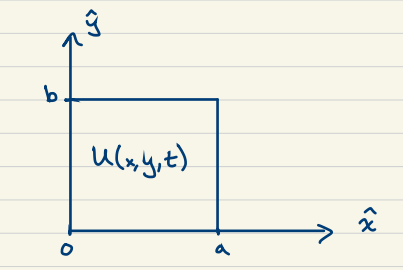
\includegraphics[height=4cm, width=7cm]{drum.PNG} 
        \label{default} 
        \end{center} 
      \end{figure} 

      \textcolor{hwColor}{
        We are required to solve the following 2-D wave equation: \\
        $
          \bigtriangledown^2 u=\dfrac{1}{v^2}\dfrac{\partial^2 u}{\partial t^2} \\
        $
      }

      \textcolor{hwColor}{
        We begin by assuming that equation is of a separable form (Otherwise what the heck are we doing here?), thus we assume a solution of the following form. \\
        \\
        $u(x,y,t)=X(x)Y(y)T(t)$ \\
        \\
        Where all functions on the RHS are there of only respective varibales. Plugging this back into our differential equation gives: \\
        \\
        $
          \bigtriangledown^2 u=\dfrac{1}{v^2}\dfrac{\partial^2 u}{\partial t^2} \\
          \\
          \dfrac{\partial^2 u}{\partial x^2}+\dfrac{\partial^2 u}{\partial y^2}=\dfrac{1}{v^2}\dfrac{\partial^2 u}{\partial t^2} \\
          \\
          X^{''}(x)Y(y)T(t)+X(x)Y^{''}(y)T(t)=\dfrac{1}{v^2}X(x)Y(y)T^{''}(t) \\
          \\
        $
        Where here we allow $X^{''}(x)=\dfrac{\partial^2 X}{\partial x}$, for example. \\
        Now dividing both sides of the equation by $u(x,y,t)$ we get: \\
        \\
        $
          \dfrac{X^{''}}{X}+\dfrac{Y^{''}}{Y}=\dfrac{1}{v^2}\dfrac{T^{''}}{T} \\
          \\
        $
        This is the equation we will be evaluating.
      }

      \textcolor{hwColor}{
        \underline{Important}: We now note, since each function in the above equation is a function of \textbf{\textit{only}} its respective varaible,
        that the \underline{only way} the above can be true is when both sides are equal to the same constant. Thus, \\
        \\
        $
          \dfrac{X^{''}}{X}+\dfrac{Y^{''}}{Y}=\dfrac{1}{v^2}\dfrac{T^{''}}{T}=\mu \\
          \\
        $
        With $\mu$ constant. This leaves us with the following systme f equations. \\
        \\
        $
          \begin{cases}
            T^{''}-\mu v^2 T=0 ~~~~~~~ (1) \\
            \dfrac{X^{''}}{X}=-\dfrac{Y^{''}}{Y}+\mu ~~~~~ (2)
          \end{cases} \\
          \\
        $
        Again, we note (2) is only true when both sides are equal to a constant. Thus, \\
        \\
        $
          \dfrac{X^{''}}{X}=\gamma=-\dfrac{Y^{''}}{Y}+\mu \\
          \\
        $
        Such that \\
        \\
        $
          X^{''}-\gamma X=0 \\
          Y^{''}-(\mu-\gamma)Y=0 \\
          \\
        $
        If we let $\sigma=\mu-\gamma$, then then second equation above can be rewritten: \\
        \\
        $
          Y^{''}-\sigma Y=0
        $ \\
        So now we are left with the following system of equations. \\
        \\
        $
          \begin{cases}
            T^{''}-\mu v^2 T=0 \\
            X^{''}- \gamma X=0 \\
            Y^{''}-\sigma Y=0
          \end{cases}
        $ \\
        With $\mu ~~ \gamma ~~ \sigma$ related by: $\sigma=\mu-\gamma$ \\
      }

      \textcolor{hwColor}{ 
        \rule{16cm}{1pt} 
      }

      \textcolor{hwColor}{
        Now let us consider one of the above equations, for example. $X^{''}-\gamma X=0$ \\
        \\
        We examine the three possilbe cases for constant $\gamma$, namely $\gamma >0 ~~~ \gamma=0 ~~~ ,and ~~~ \gamma <0$ \\
        \\
        Let $\gamma=\alpha^2$, then for $\gamma > 0$, we have $\rightarrow X^{''}-\alpha^2 X=0 ~~~~ (3)$ \\
        \\
        Where we will assume the following solution: \\
        $
          \begin{cases}
            X(x)=Ae^{\alpha x}+B e^{-\alpha x} \\
            \\
            X^{'}(x)=\alpha Ae^{\alpha x}- \alpha B e^{-\alpha x} \\
            \\
            X^{''}(x)=\alpha^2 Ae^{\alpha x}+\alpha^2 Be^{-\alpha x}
          \end{cases} \\
        $
        \\
        This is where we can see this satisfies (3).
      }

      \textcolor{hwColor}{
        For $\gamma=0$, we have $X^{''}-(0)X=0 \longrightarrow X^{''}=0$ \\
        \\
        This we will denote the \underline{trivial solution} and discard for now. \\
        \\
      }

      \textcolor{hwColor}{ 
        \rule{16cm}{1pt} 
      }

      \textcolor{hwColor}{
        For $\gamma<0$, we have \\
        $
          X^{''}+\alpha^2 X=0 ~~~~ (4) \\
          \\
        $
        Where we will assume a solution of the following form: \\
        \\
        $X(x)=Ccos(\alpha x)+Dsin(\alpha x)$ \\
        \\
        Thus,\\
        \\
        $
          \begin{cases}
            X^{'}(x)=-C\alpha sin(\alpha x)+D \alpha cos(\alpha x) \\
            \\
            X^{''}(x)=-C \alpha^2 cos(\alpha x)-D \alpha^2 sin(\alpha x)
          \end{cases} \\
        $
        Which we can see satisfies (4).
      }

      \textcolor{hwColor}{ 
        \rule{16cm}{1pt} 
      }

      \textcolor{hwColor}{ 
        Thus our general solution for $X(x)$ will be the following: \\
        $
          X(x)=\begin{cases}
            Ae^{\alpha x}+Be^{-\alpha x} ~~~~~~~~~~~~~, \gamma=\alpha^2 > 0 \\
            \\
            0 ~~~~~~~~~~~~~~~~~~~~~~~~~~~~~~~, \gamma=\alpha^2=0 \\
            \\
            Ccos(\alpha x)+Dsin(\alpha x) ~~~, \gamma=\alpha^2 < 0
          \end{cases}
        $
      }

      \textcolor{hwColor}{ 
        \rule{16cm}{1pt} 
      }

      \textcolor{hwColor}{ 
        An identical argument can be made for functions $Y(y)$ and $T(t)$, with special care given to the extra
        contant $v^2$ in our $T(t)$ equation. \\
        $
        Y(y)=\begin{cases}
          Ee^{\beta y}+Fe^{-\beta y} ~~~~~~~~~~~~~, \sigma=\beta^2 > 0 \\
          \\
          0 ~~~~~~~~~~~~~~~~~~~~~~~~~~~~~~~, \sigma=\beta^2=0 \\
          \\
          Gcos(\beta y)+Hsin(\beta y) ~~~, \sigma=\beta^2 < 0
        \end{cases}
        $ \\
        \\
      }

      
      \textcolor{hwColor}{ 
        $
        T(t)=\begin{cases}
          Ie^{\delta v t}+Je^{-\delta v t} ~~~~~~~~~~~~~, \mu=\delta^2 > 0 \\
          \\
          0 ~~~~~~~~~~~~~~~~~~~~~~~~~~~~~~~, \mu=\delta^2=0 \\
          \\
          Kcos(\delta v t)+Lsin(\delta v t) ~~~, \mu=\delta^2 < 0
        \end{cases}
        $ \\
        \\
      }

      \textcolor{hwColor}{ 
        Where our most general solution is again. \\
        \\
        $u(x,y,t)=X(x)Y(y)T(t)$
      }


    \item Impose that the edges of the drum are fixed at all times and write the updated solution that takes these conditions into account.

      \textcolor{hwColor}{ 
        We assume that the edges of the drum are fixed. The wave equation for a transverse wave traveling on a 2D-wave is given by: \\
        \\
        $
          \dfrac{\partial^2 z}{\partial t^2}=\dfrac{\delta}{\sigma}\left[\dfrac{\partial^2 z}{\partial x^2}+\dfrac{\partial^2 z}{\partial y^2}\right] \\
          \\
          \omega^2=\dfrac{\delta}{\sigma}(k^2_x+k^2_y) \\
          \\
          z(x,y,t)=Asin(k_x x)sin(k_y y)e^{-i\omega t} \\
          \\
        $
        The solution is found by taking the boundry condition into account: \\
        \\
        $
          z(0,0,t)=0 \rightarrow A=0 \\
          \\
          \Longrightarrow \dfrac{dz}{dt}=A\omega sin(k_x x)sin(k_y y)
        $
      }
    
    \end{enumerate}


  \item  Continuing the problem above, now impose that the drumhead is described at time $t=0$ by the following conditions: 
      $$
      U(x, y, 0) = \frac{\epsilon}{a^2 b^2} xy(a-x)(b-y)~, 
      $$
      $$
      \frac{\partial U}{\partial t} \bigg|_{t=0}=0
      $$
      simplify, and write the final solution. \\

      (NOTE:  If everything was done correctly, after rearranging and simplifying, you should obtain the following expression: 
      $$
      U(x,y,t)= \epsilon \left(\frac{2}{\pi} \right)^6 \sum^{\infty}_{m=1} \sum^{\infty}_{n=1} \frac{1}{(2m-1)^3( 2n -1)^3} \\
      \times \sin\left( \frac{(2m-1) \pi x}{a} \right) \sin \left( \frac{(2n-1) \pi y}{b}  \right)  \cos(\omega_{mn} t)
      $$~, where
      $$
      \omega^2_{mn}= \pi^2 v^2 \left(  \frac{(2m-1)^2 }{a^2} +  \frac{(2n-1)^2}{ b^2}    \right)~~,~~m,n=1,2,3,...  ) 
      $$

  \end{enumerate}

\end{document}
